%!TeX root=../tese.tex
%("dica" para o editor de texto: este arquivo é parte de um documento maior)
% para saber mais: https://tex.stackexchange.com/q/78101/183146

%% ------------------------------------------------------------------------- %%
\chapter{Interpretação geométrica de buscas em ABBs}
\label{cap:geometria}

Neste capítulo explicaremos a visão geométrica proposta por Demaine, Harmon, Iacono e Pătrașcu \cite{geometry_of_bst}, o que são conjuntos de pontos arboreamente satisfeitos e como interpretar de maneira geométrica algoritmos de busca em ABBs.

\section{Conjuntos arboreamente satisfeitos}

Chamamos dois pontos $a$ e $b$ de \textit{ortogonalmente colineares} se $a$ e $b$ estão na mesma linha horizontal ou vertical. Se $a$ e $b$ não são ortogonalmente colineares, denotamos por \textit{$\{a,b\}$-retângulo} o retângulo ortogonal que tem $a$ e $b$ como vértices.

Um par de pontos $\{a,b\}$ de um conjunto de pontos $P$ é \textit{arboreamente satisfeito} se $a$ e $b$ são ortogonalmente colineares ou se há pelo menos um ponto do conjunto \( P \setminus \{a,b\} \) que está dentro da região delimitada pelo \{a,b\}-retângulo, incluindo seu perímetro. Um conjunto $P$ de pontos é \textit{arboreamente satisfeito} se todos os pares de pontos do conjunto são arboreamente satisfeitos. Veja a Figura~\ref{fig:geometria-inicial}.

\begin{figure}[h!]
    \centering
    \begin{minipage}[b]{0.45\textwidth}
        \centering
        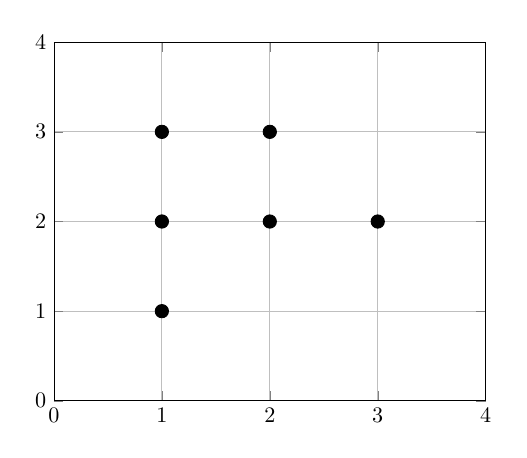
\begin{tikzpicture}[scale=0.8]
        \begin{axis}[
            grid=major,
            xmin=0, xmax=4,
            ymin=0, ymax=4,
            xtick={0,1,2,3,4},
            ytick={0,1,2,3,4}
        ]
        \addplot[only marks, mark=*, mark size=3pt] coordinates {
            (1,1)
            (1,2)
            (1,3)
            (2,2)
            (2,3)
            (3,2)
        };
        \end{axis}
        \end{tikzpicture}
    \end{minipage}\hfill
    \begin{minipage}[b]{0.45\textwidth}
        \centering
        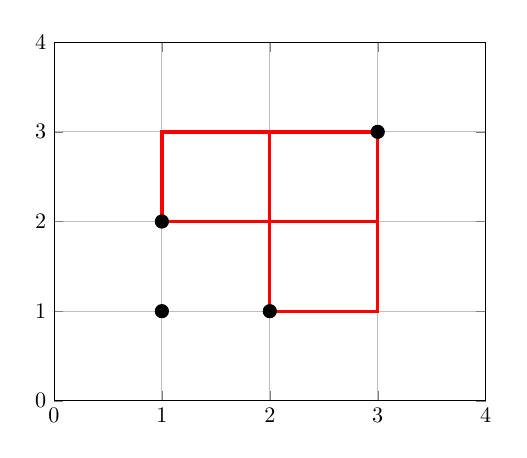
\begin{tikzpicture}[scale=0.8]
        \begin{axis}[
            grid=major,
            xmin=0, xmax=4,
            ymin=0, ymax=4,
            xtick={0,1,2,3,4},
            ytick={0,1,2,3,4}
        ]
        \addplot[only marks, mark=*, mark size=3pt] coordinates {
            (1,1)
            (1,2)
            (2,1)
            (3,3)
        };
        \addplot[
            color=red,
            line width=1.5pt
        ]
        coordinates {
            (2,1)
            (3,1)
            (3,3)
            (2,3)
            (2,1)
        };
        \addplot[
            color=red,
            line width=1.5pt
        ]
        coordinates {
            (1,2)
            (3,2)
            (3,3)
            (1,3)
            (1,2)
        };
        \end{axis}
        \end{tikzpicture}
    \end{minipage}
    \caption{À esquerda, um conjunto $P$ de pontos arboreamente satisfeito. À direita, um conjunto $P$ de pontos com dois pares de pontos arboreamente insatisfeitos com seus retângulos destacados.}
\label{fig:geometria-inicial}
\end{figure}

\begin{lemma}
\label{lem:pontos_em_arestas_incidentes}
Em um conjunto arboreamente satisfeito $P$, para todo par de pontos $\{a,b\}$ não ortogonalmente colineares, há sempre pelo menos um ponto de \( P \setminus \{a,b\} \) que está em um dos lados do $\{a,b\}$-retângulo que incide em $a$, e há sempre também pelo menos um ponto de \( P \setminus \{a,b\} \) que está em um dos lados do $\{a,b\}$-retângulo que incide em $b$.
\end{lemma}

\begin{figure}
    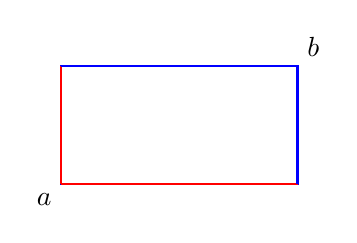
\begin{tikzpicture}[scale=1.5]
        \draw[blue, thick] (0,0) rectangle (2,1);
        
        \node at (0,0) [below left] {$a$};
        \node at (2,1) [above right] {$b$};
        
        \draw[red, thick] (0,0) -- (0,1);
        \draw[red, thick] (0,0) -- (2,0);
        \draw[blue, thick] (2,1) -- (0,1);
        \draw[blue, thick] (2,1) -- (2,0);
    \end{tikzpicture}
    \caption{O $\{a,b\}$-retângulo. Em vermelho estão destacados os lados do retângulo que incidem em $a$ e em azul estão destacados os lados que incidem em $b$.}
\end{figure}

\begin{proof}
    %Provaremos essa propriedade a partir de uma indução no número de pontos no interior dos retângulos. Seja $P$ o conjunto de pontos arboreamente satisfeito sendo analisado e sejam $a$ e $b$ dois pontos de $P$.
    %O caso base da indução é quando não há pontos de $P$ no interior do $\{a,b\}$-retângulo. Se existir algum ponto de $P \setminus \{a,b\}$ em um dos vértices do $\{a,b\}$-retângulo, então a propriedade é valida. Caso contrário, é necessário analisar as arestas do $\{a,b\}$-retângulo. Assuma sem perda de generalidade que $b$ está acima e a direita de $a$. 
    %Denotemos por $c$ o ponto de $P$ mais a esquerda na aresta horizontal superior. Denotemos por $d$ o ponto de $P$ mais abaixo na aresta vertical direita.
    %Se $c$ for diferente de $b$, então obrigatoriamente existe um ponto de $P$ com mesma coordenada $x$ de $c$ na aresta horizontal inferior, pois, caso contrário, $c$ e o ponto com maior coordenada $x$ na aresta horizontal inferior que possua coordenada $x$ menor que $c$ formariam um par de pontos arboreamente insatisfeito.
    %Se $c$ for igual a $b$, então obrigatoriamente $d$ é diferente de $b$, e pelo mesmo argumento geométrico, deve existir um ponto de $P$ com mesma coordenada $y$ na aresta vertical esquerda, pois caso contrário, o ponto $d$ e o ponto com maior coordenada $y$ na aresta vertical esquerda que possua coordenada $y$ menor que $d$ formariam um par de pontos arboreamente insatisfeito.

    Vamos provar por indução em $k$ que, todo $\{a,b\}$-retângulo com $k$ pontos em seu interior satisfaz a propriedade do Lema.

    Para $k = 0$, todo $\{a,b\}$-retângulo possui um ponto de $P \setminus \{a,b\}$ em um de seus vértices ou possui dois pontos de $P \setminus \{a,b\}$ em seu perímetro alinhados verticalmente ou horizontalmente. Caso o $\{a,b\}$-retângulo possua um ponto de $P \setminus \{a,b\}$ em um de seus vértices, então a propriedade é válida. Caso o $\{a,b\}$-retângulo possua dois pontos de $P \setminus \{a,b\}$ em seu perímetro alinhados verticalmente ou horizontalmente, então um desses pontos está em um dos lados do $\{a,b\}$-retângulo que incide em $a$ e o outro está em um dos lados do $\{a,b\}$-retângulo que incide em $b$, satisfazendo a propriedade do lema.

    Suponha agora que $k > 0$ e que a propriedade vale para todo retângulo com menos que $k$ pontos de $P$ em seu interior. Seja $e$ um ponto de $P$ no interior do $\{a,b\}$-retângulo. O $\{a,e\}$-retângulo e o $\{e,b\}$-retângulo são retângulos de $P$ com menos que $k$ pontos, logo a propriedade vale para esses retângulos. Como os lados do $\{a,b\}$-retângulo que incidem em $a$ contém os lados do $\{a,e\}$-retângulo que incidem $a$ e os lados do $\{a,b\}$-retângulo que incidem em $b$ contém os lados do $\{e,b\}$-retângulo que incidem $b$, então se a propriedade vale também para o $\{a,b\}$-retângulo.    
\end{proof}

\section{Visão geométrica de buscas}

No modelo de computação adotado, para realizar um acesso em uma ABB, o algoritmo de busca inicia o nó corrente na raiz da ABB. Em seguida, percorre a árvore descendo para o filho apropriado por meio de comparações até alcançar a chave procurada.

Dada uma sequência $X = (x_{1},\ldots,x_{m})$ de $m$ acessos às chaves $1,2,\ldots,n$, é possível ilustrar essa sequência $X$ de maneira gráfica em um plano cartesiano da seguinte forma: o eixo $x$ representará as chaves armazenadas na ABB e o eixo $y$ representará os índices $i = 1,2,\ldots,m$, que interpretamos como o tempo. Denotaremos por $P_X$ esse conjunto de pontos. Assim, um ponto de coordenada ($x$,$i$) representa a busca da chave $x$ na ABB no instante de tempo $i$, ou seja, representa $x_i$. Veja o exemplo da Figura~\ref{fig:busca_padrao}.

\begin{figure}
    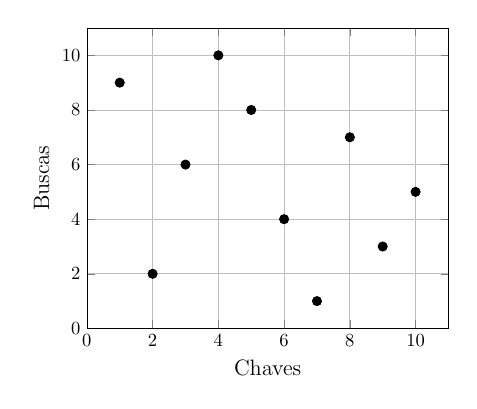
\begin{tikzpicture}[scale=0.67]
        \begin{axis}[
            xlabel={Chaves},
            ylabel={Buscas},
            xlabel style={font=\large},
            ylabel style={font=\large},
            grid=major,
            xmin=0, xmax=11,
            ymin=0, ymax=11,
            xtick={0,2,4,6,8,10},
            ytick={0,2,4,6,8,10}
        ]
        \addplot[only marks, mark=*, mark size=2.5pt] coordinates {
            (1,9)
            (2,2)
            (3,6)
            (4,10)
            (5,8)
            (6,4)
            (7,1)
            (8,7)
            (9,3)
            (10,5)
        };
        \end{axis}
    \end{tikzpicture}
    \caption{Gráfico representando a sequência (7, 2, 9, 6, 10, 3, 8, 5, 1, 4) de acessos.}
\label{fig:busca_padrao}
\end{figure}

A \textit{visão geométrica da execução de um algoritmo de busca em ABB} para uma sequência $X = (x_{1},\ldots,x_{m})$ de buscas, de maneira similar, é o conjunto $P$ de pontos na forma ($x$,$i$) tal que $x$ foi uma das chaves visitadas durante a busca pela chave $x_i$. Para cada $i \in \{1,\ldots,m\}$, os pontos de $P$ pertencentes a reta $y = i$ representam as chaves dos nós visitados durante a busca por $x_i$. Veja a Figura~\ref{fig:traducao-busca-em-ASS}.

\begin{figure}[h!]
    \centering
    \begin{minipage}[b]{0.34\textwidth}
        \centering
        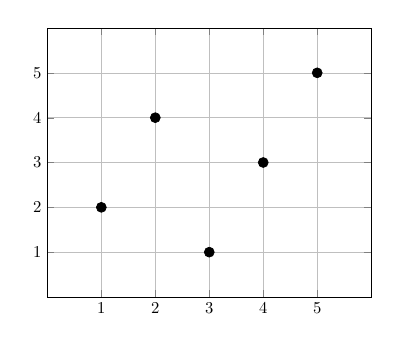
\begin{tikzpicture}[scale=0.6]
        \begin{axis}[
            grid=major,
            xmin=0, xmax=6,
            ymin=0, ymax=6,
            xtick={1,2,3,4,5},
            ytick={1,2,3,4,5}
        ]
        \addplot[only marks, mark=*, mark size=3pt] coordinates {
            (3,1)
            (1,2)
            (4,3)
            (2,4)
            (5,5)
        };
        \end{axis}
        \end{tikzpicture}
    \end{minipage}\hfill
    \begin{minipage}[b]{0.33\textwidth}
        \centering
        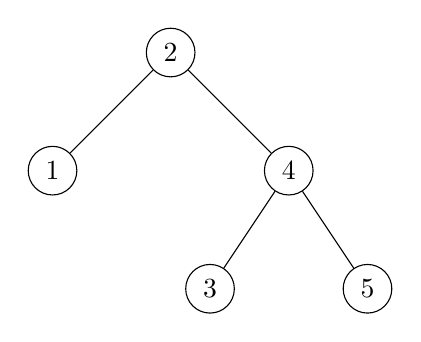
\begin{tikzpicture}
            [node/.style={circle,draw,minimum size=1.5em}]
            \node[node] (A) at (-1.5,-1.5) {$1$};
            \node[node] (B) at (0,0) {$2$};
            \node[node] (C) at (0.5,-3) {$3$};
            \node[node] (D) at (1.5,-1.5) {$4$};
            \node[node] (E) at (2.5,-3) {$5$};
            
            \draw (A) -- (B);
            \draw (B) -- (D);
            \draw (C) -- (D);
            \draw (E) -- (D);
          \end{tikzpicture}
    \end{minipage}\hfill
    \begin{minipage}[b]{0.33\textwidth}
        \centering
        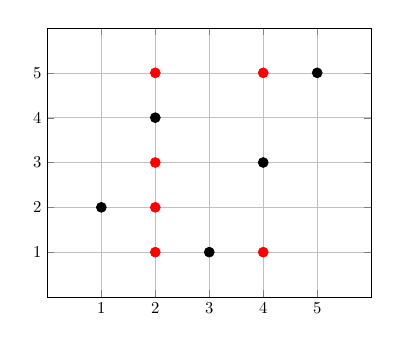
\begin{tikzpicture}[scale=0.6]
            \begin{axis}[
                grid=major,
                xmin=0, xmax=6,
                ymin=0, ymax=6,
                xtick={1,2,3,4,5},
                ytick={1,2,3,4,5}
            ]
            \addplot[only marks, mark=*, mark size=3pt] coordinates {
                (3,1)
                (1,2)
                (4,3)
                (2,4)
                (5,5)
            };
            \addplot[color=red, only marks, mark=*, mark size=3pt] coordinates {
                (2,1)
                (4,1)
                (2,2)
                (2,3)
                (2,5)
                (4,5)
            };
            \end{axis}
            \end{tikzpicture}
    \end{minipage}
    \caption{À esquerda, o conjunto de pontos que representa a sequência $X = (3,1,4,2,5)$. No meio, uma possível ABB com as chaves \{1,2,\ldots,5\}. À direita, o conjunto correspondente aos nós da ABB ao centro, visitados pelo algoritmo de busca que não efetua rotações. Os pontos pretos são os nós da sequência $X$ de acessos e os pontos vermelhos são o restante dos nós visitados durante cada um desses acessos. Note que o conjunto de pontos à esquerda não é arboreamente satisfeito, mas o conjunto à direita é.}
\label{fig:traducao-busca-em-ASS}
\end{figure}

\begin{lemma} A visão geométrica de qualquer execução de um algoritmo de busca em ABB no modelo de computação adotado é um conjunto de pontos arboreamente satisfeitos.
\label{lema:visao_geometrica_vira_ASS}
\end{lemma}

\begin{proof}
Seja $P$ a visão geométrica da execução de um algoritmo de busca em uma ABB $T$ para alguma sequência $X$ de buscas.
Suponha, por contradição, que $P$ não é um conjunto arboreamente satisfeito. Dessa maneira, há pelo menos um par $\{p,q\}$ de pontos de $P$ que não é arboreamente satisfeito, onde $p = (a,i)$ e $q = (b,j)$. Assumiremos sem perda de generalidade que $i < j$ e $a < b$.

Seja $r$ o nó de $T$ com chave $a$ e seja $s$ o nó de $T$ com chave $b$.

Dois lados do $\{p,q\}$-retângulo terão um papel a seguir na prova. São eles:
\begin{itemize}
    \item $\ell_1$ = \{$(x,y)$ | $a \leq x < b$ e $y = j$\}, e
    \item $\ell_2$ = \{$(x,y)$ | $x = b$ e $i \leq y < j$\},
\end{itemize}
onde, dentro do contexto da ABB $T$, $\ell_1$ representa as visitas aos nós com chave no intervalo $[a,b)$ no instante $j$ e $\ell_2$ representa as visitas ao nó $s$ entre os instantes de tempo $i$ e $j$.

Como $\{p,q\}$ é um par de pontos arboreamente insatisfeito, nota-se que não há nenhum ponto de $P$ tanto nas bordas quanto no interior do $\{p,q\}$-retângulo. Logo, $(\ell_1 \cup \ell_2) \cap P = \emptyset$.

Sejam $c_1$ e $c_3$ respectivamente as chaves de dois nós $n_1$ e $n_3$ de uma ABB com $c_1 \leq c_3$. Se $n_2$ é o ancestral comum mais profundo dos nós $n_1$ e $n_3$ e sua chave é $c_2$, então sabemos que $c_1 \leq c_2 \leq c_3$ e, mais importante, $n_2$ é ancestral dos nós $n_1$ e $n_3$ nesta ABB, e assim os nós $n_1$ e $n_3$ têm profundidade maior ou igual a $n_2$. Logo, $n_2$ está no caminho da raiz desta ABB até qualquer nó com chave no intervalo $[c_1,c_3]$. Em outras palavras, para visitar qualquer nó da ABB com chave no intervalo $[c_1,c_3]$, é necessário visitar o ancestral comum mais profundo entre $n_1$ e $n_3$, que neste caso é $n_2$.

\begin{center}
\begin{minipage}[t]{0.6\textwidth}
    Seja $c$ a chave do ancestral comum mais profundo de $r$ e $s$ em $T$ imediatamente antes da busca $i$. Seja $d$ a chave do ancestral comum mais profundo de $r$ e $s$ em $T$ imediatamente antes da busca $j$.
    
    Como $\ell_1 \cap P = \emptyset$, então obrigatoriamente $d = b$. Por outro lado, como $\ell_2 \cap P = \emptyset$, temos que $c \neq b$ e, em algum instante $h$, com $i \leq h < j$, o nó $s$ teve que ser visitado para ser rotacionado e se tornar o ancestral comum mais profundo entre $r$ e $s$ no instante imediatamente antes de $j$, logo $\ell_2 \cap P \neq \emptyset$, uma contradição.
\end{minipage}\hfill
\begin{minipage}[t]{0.4\textwidth}
    \centering
    \vspace{-0.65cm}
    \begin{figure}[H]
        \centering
        \begin{adjustbox}{valign=t}
        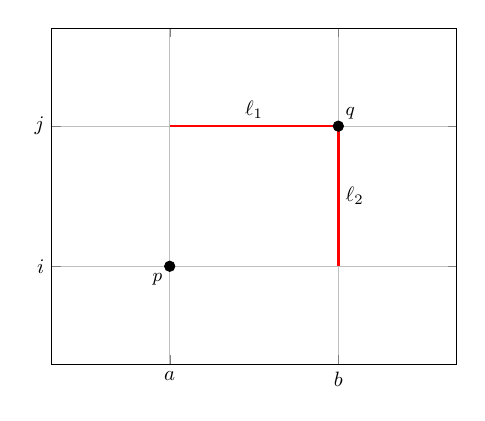
\begin{tikzpicture}[scale=0.75]
        \begin{axis}[
            grid=major,
            xmin=0.3, xmax=2.7,
            ymin=0.3, ymax=2.7,
            xtick={1,2},
            ytick={1,2},
            xlabel style={at={(axis description cs:0.5,-0.08)}, anchor=center}, % Ajusta a posição do rótulo do eixo x
            ylabel style={at={(axis description cs:-0.08,0.5)}, anchor=center},
            xticklabels={$a$,$b$}, % Define os rótulos do eixo x
            yticklabels={$i$,$j$} % Define os rótulos do eixo y
        ]

        \addplot[only marks, mark=*, mark size=2.5pt] coordinates {
            (1,1)
            (2,2)
        };

        \addplot[red, very thick] coordinates {
            (1,2)
            (2,2)
        };

        \addplot[red, very thick] coordinates {
            (2,2)
            (2,1)
        };
        \node at (axis cs:1,1) [anchor=north east, fill=white, font=\small] {$p$};
        \node at (axis cs:2,2) [anchor=south west, fill=white, font=\small] {$q$};
        \node at (axis cs:1.5,2) [anchor=south, font=\normalsize] {$\ell_1$};
        \node at (axis cs:2,1.5) [anchor=west, font=\normalsize] {$\ell_2$};
        \end{axis}
        \end{tikzpicture}
        \end{adjustbox}
        \label{fig:tikz-captions}
    \end{figure}
\end{minipage}
\end{center}
\vspace{-0.7cm}
\end{proof}

A partir daqui, consideraremos apenas pontos $(x,y)$ em que $x$ e $y$ são inteiros, $1 \leq x \leq n$ e $1 \leq y \leq m$.

\begin{lemma}Qualquer conjunto de pontos arboreamente satisfeito representa a execução de um algoritmo de busca em ABB no modelo de computação adotado.
\label{lema:ASS_vira_visao_geometrica}
\end{lemma}

\begin{proof}\label{prova:ASS}
Usaremos um tipo de árvore binária de busca denominada \textit{treap}. Os nós de uma treap possuem dois campos, um chamado chave e outro chamado prioridade. A treap mantém duas propriedades: a propriedade de ordem de árvores binárias de busca em relação às chaves e a propriedade de heap em relação às prioridades. Assim, todo nó de uma treap possui chave maior que os nós da sua subárvore esquerda e chave menor que os nós da sua subárvore direita. Além disso, os nós da treap obedecem à propriedade de heap, que pode ser de dois tipos: se for um heap máximo, cada nó terá prioridade maior ou igual a de seus filhos; se for um heap mínimo, cada nó terá prioridade menor ou igual a de seus filhos.

Seja $P$ um conjunto de pontos arboreamente satisfeito. Denotaremos por $N(h,i)$ a coordenada $y$ do ponto mais baixo de $P$ que possui coordenadas $x = h$ e $y > i$. Caso não exista tal ponto, definiremos $N(h,i) = \infty$. Assim, 
\begin{center}
    $N(h,i) = \min\{y : (h,y) \in P \text{ e } y > i\}$,
\end{center}
onde o mínimo sobre o conjunto vazio é $\infty$.

É possível criar uma treap com as chaves $1,\ldots,n$ que é um heap mínimo nas prioridades a partir de $P$. Para cada $j \in \{1,\ldots,n\}$, adicione um nó na forma ($j$, $N(j,0)$), ou seja, adicione um nó com chave $j$ e prioridade $N(j,0)$. Essa é a nossa treap inicial.

Com essa treap criada, nota-se que já temos uma ABB que possui $n$ nós. Se conseguirmos descrever uma maneira de, para cada instante de tempo $h \in \{1,\ldots,m\}$, visitarmos todos os nós com chave $z$ tais que que $(z,h) \in P$ e reestruturamos a treap de maneira a manter sua estrutura sem visitar nós extras, então descrevemos uma execução de um algoritmo offline de busca em uma ABB no modelo de computação adotado.

Primeiramente, note que os nós com prioridade mínima induzem uma subárvore da treap que contém a raiz.
Seja $i$ essa prioridade mínima. Os nós com prioridade $i$ serão visitados no instante $i$ e terão sua prioridade alterada apenas considerando essa subárvore. Queremos mostrar que, ao fazer tais alterações nas prioridades no instante $i$ e reorganizar a treap dessa maneira, a treap toda continua satisfazendo a propriedade de heap.

Vamos supor, por contradição, que há um nó $q$ cuja prioridade é menor que de seu pai $p$ na treap após as modificações do instante $i$. Isso só pode ocorrer se $p$ estiver dentro da subárvore dos nós visitados no instante $i$ e $q$ não estiver nessa subárvore. Seja $a$ a chave de $p$ e $b$ a chave de $q$ e assumiremos sem perda de generalidade que $a < b$. Assim, $N(a,i) > N(b,i)$. Veja a Figura~\ref{fig:representacao_grafica}.

%que há dois nós, $p$ com chave $a$ e $q$ com chave $b$ ($a \neq b$), tal que o nó $p$ está contido na subárvore dos nós visitados no instante de tempo $i$ e o nó $q$ não foi visitado no instante de tempo $i$ e sua prioridade é menor que . Assim, $N(a,i) > N(b,i)$. Assumiremos sem perda de generalidade que $a < b$ e que $p$ é pai de $q$ durante o instante de tempo $i$. Veja a Figura~\ref{fig:representacao_grafica}.

\begin{figure}[H]
    \begin{tikzpicture}[scale=1.1]
        \coordinate (A) at (0, 0);
        \coordinate (B) at (3, 0);
        \coordinate (C) at (1.5, 2.6);
    
        \draw (A) -- (B) -- (C) -- cycle;
    
        \path (A) ++(0,1) coordinate (start);
        \path (start) ++(3,0.7) coordinate (end);
        \draw[dashed] (start) -- (end) node[midway,below] {};
    
        \path (start) ++(1.5,0.57) coordinate (x);
        \path (start) ++(1.7,0.2) coordinate (y);

        \begin{scope}
            \clip (A) -- (B) -- (C) -- cycle; % Clipping para definir a área do triângulo
            \fill[pattern=vertical lines] (A) -- (C) -- (end) -- (start) -- cycle; % Preenchimento hachurado
        \end{scope}
    
        %\filldraw (x) circle (2pt) node[anchor=south] {};
        %\filldraw (y) circle (2pt) node[anchor=north] {};
    
        \draw[red, thick] (x) -- (y);

        \filldraw (x) circle (1.5pt) node[anchor=south] {$p$};
        \filldraw (y) circle (1.5pt) node[anchor=north] {$q$};

        \draw[->, black] (1.8,1.8) -- (2.5,2) node[pos=1, right] {Nós visitados no instante de tempo $i$};
    \end{tikzpicture}
    \caption{Representação da situação descrita. O triângulo é uma representação simplificada de uma ABB. A área destacada representa todos os nós acessados no instante de tempo $i$. O nó $q$ não foi visitado nesse instante de tempo.}
\label{fig:representacao_grafica}
\end{figure}
De maneira informal, os nós $p$ e $q$ são nós pai-filho. Durante o instante de tempo $i$, $p$ será visitado pelo algoritmo de busca e $q$ não. Após o instante $i$, queremos visitar o nó $q$ pela primeira vez no instante $j = N(b,i)$ antes de fazer qualquer outra visita ao nó $p$, porém isso é impossível. Vamos mostrar que, neste caso, $P$ não era um conjunto arboreamente satisfeito.

Os lados a seguir terão um papel na prova e estão representados na Figura~\ref{fig:area_delimitada}. São eles:
\begin{itemize}
    \item $\ell_1$ = \{$(x,y)$ | $x = a$ e $i < y \leq j$\}, e
    \item $\ell_2$ = \{$(x,y)$ | $a < x \leq b$ e $y = i$\},
\end{itemize}
onde $\ell_1 \cap P = \emptyset$, pois o nó $p$ não é visitado entre os instantes de tempo $i+1$ e $j$ já que $N(a,i) > j$, e $\ell_2 \cap P$ representa todas as visitas aos nós com chave no intervalo $(a,b]$ no instante de tempo $i$.

Denotemos por $r$ o ponto com coordenadas $(a,i)$ e por $s$ o ponto com coordenadas $(b,j)$. De acordo com a suposição feita, ambos estes pontos pertencem a $P$.
\begin{figure}
    \centering
    \begin{adjustbox}{valign=t, raise=-25pt} % Alinha o gráfico ao topo da caixa
    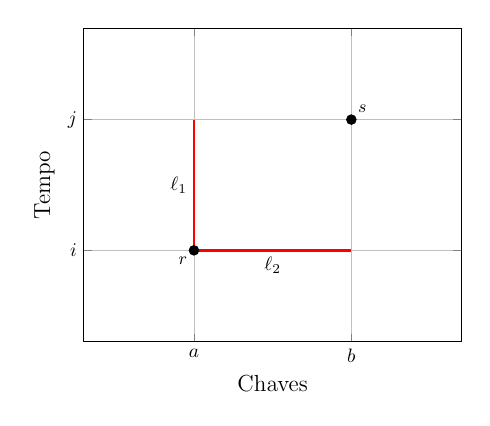
\begin{tikzpicture}[scale=0.7]
    \begin{axis}[
        xlabel={Chaves},
        ylabel={Tempo},
        grid=major,
        xmin=0.3, xmax=2.7,
        ymin=0.3, ymax=2.7,
        xlabel style={font=\large},
        ylabel style={font=\large},
        xtick={1,2},
        ytick={1,2},
        %xlabel style={at={(axis description cs:0.5,-0.08)}, anchor=center}, % Ajusta a posição do rótulo do eixo x
        %ylabel style={at={(axis description cs:-0.08,0.5)}, anchor=center},
        xticklabels={$a$,$b$}, % Define os rótulos do eixo x
        yticklabels={$i$,$j$} % Define os rótulos do eixo y
    ]

    \addplot[only marks, mark=*, mark size=2.5pt] coordinates {
        (1,1)
        (2,2)
    };

    \addplot[red, very thick] coordinates {
        (1,1)
        (1,2)
    };

    \addplot[red, very thick] coordinates {
        (1,1)
        (2,1)
    };

    % Adiciona rótulos aos pontos
    \node at (axis cs:1,1) [anchor=north east, fill=white, font=\small] {$r$};
    \node at (axis cs:2,2) [anchor=south west, fill=white, font=\small] {$s$};

    \node at (axis cs:1,1.5) [anchor=east, font=\normalsize] {$\ell_1$};
    \node at (axis cs:1.5,1) [anchor=north, font=\normalsize] {$\ell_2$};

    \end{axis}
    \end{tikzpicture}
    \end{adjustbox}
    \caption{Representação no conjunto $P$ da situação descrita.}
\label{fig:area_delimitada}
\end{figure}

Como $r,s \in P$, então $\{r,s\}$ representa um par de pontos arboreamente satisfeito. De acordo com o Lema~\ref{lem:pontos_em_arestas_incidentes}, como $r$ e $s$ não são ortogonalmente colineares, há pelo menos um outro ponto de $P$ em alguma das arestas do $\{r,s\}$-retângulo que incide em $r$. Como $\ell_1 \cap P = \emptyset$, então $\ell_2 \cap P \neq \emptyset$. Assim, há um ponto de $P$ no lado $\ell_2$ e, consequentemente, algum nó com chave no intervalo $(a,b]$ deve ter sido visitado durante o instante de tempo~$i$.

Como $q$ é filho direito de $p$, então qualquer nó de chave no intervalo ($a,b$) no instante de tempo $i$, pela propriedade da ordenação de ABBs, está na subárvore esquerda do nó $q$. Assim, para visitar qualquer nó com chave neste intervalo é necessário visitar ambos os nós $p$ e $q$, porém pela hipótese o nó $q$ não é visitado em $i$, logo $\ell_2 \cap P = \emptyset$, uma contradição.

Assim, nota-se que a reestruturação da treap da maneira proposta é sempre válida em conjuntos de pontos arboreamente satisfeitos e tal reestruturação descreve um algoritmo offline que converte um conjunto de pontos arboreamente satisfeitos em uma execução de um algoritmo de busca em ABB dentro do modelo de computação adotado.
\end{proof}

%Ao longo dessa pesquisa, uma série de conjuntos de pontos foram analisados. 
Verificar se um conjunto de pontos é arboreamente satisfeito é demorado se feito à mão. Assim, com o intuito de automatizar e garantir que um conjunto de pontos sendo analisado é arboreamente satisfeito, implementamos a treap proposta na Demonstração~\ref{prova:ASS}. %Essa treap executa um desce heap na raiz múltiplas vezes em cada instante de tempo e detecta se a propriedade de heap mínimo foi violada em algum momento. 
Se a propriedade não for violada, o código imprime a árvore correspondente a cada instante de tempo, caso a propriedade seja violada, o código imprime todas as árvores correspondentes aos instantes de tempo anteriores ao da violação e imprime o par de pontos que é arboreamente insatisfeito. A implementação pode ser vista \href{https://github.com/BrunoArmondBraga/TCC/blob/main/src/ValidAss.cpp}{aqui}.

É importante notar que essa interpretação geométrica é muito útil para entender buscas em ABBs de maneira simplificada. Essa abordagem convenientemente oculta as rotações da ABB e leva em consideração apenas os nós visitados durante as buscas. É bastante impressionante que a disposição exata dos nós de uma ABB não é uma informação essencial para a análise e pode ser reconstruída a partir dos nós visitados.

Os resultados desse capítulo implicam que o tamanho do menor conjunto de pontos arboreamente satisfeito que contém $P_X$ é exatamente OPT($X$). No próximo capítulo apresentaremos um algoritmo guloso que dada uma sequência de buscas $X$ produz um conjunto arboreamente satisfeito que contém $P_X$ tentando minimizar o tamanho desse conjunto. Esse algoritmo é online.